\documentclass[tikz,border=2pt]{standalone}
\usepackage{amsmath,amssymb}
\usepackage{tikz}
\usetikzlibrary{arrows.meta}

\begin{document}
% N x N is countably infinite: the zig-zag path visits every pair (i, j) exactly once, giving
% a bijection with N. The same trick lists the positive rationals.
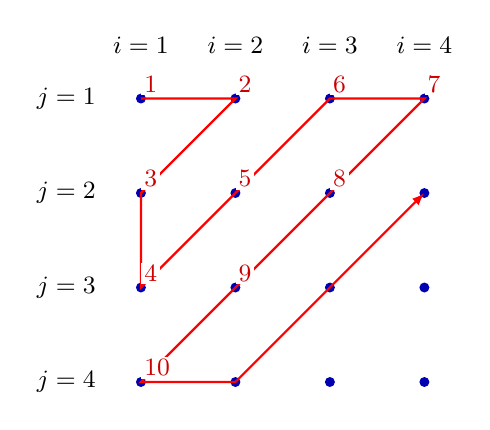
\begin{tikzpicture}[every node/.style={font=\small}, >={Latex[length=1.6mm]}]
	\foreach \i in {1,...,4} {\foreach \j in {1,...,4} {\fill[blue!70!black] (\i*1.2,-\j*1.2) circle (1.8pt);}}
	\foreach \i in {1,...,4} {\node[above] at (\i*1.2,-0.75) {$i=\i$};}
	\foreach \j in {1,...,4} {\node[left] at (0.75,-\j*1.2) {$j=\j$};}
	\draw[red, thick, ->] (1.2,-1.2) -- (2.4,-1.2) -- (1.2,-2.4) -- (1.2,-3.6) -- (2.4,-2.4) -- (3.6,-1.2) -- (4.8,-1.2) -- (3.6,-2.4) -- (2.4,-3.6) -- (1.2,-4.8) -- (2.4,-4.8) -- (3.6,-3.6) -- (4.8,-2.4);
	\foreach \n/\x/\y in {1/1/1, 2/2/1, 3/1/2, 4/1/3, 5/2/2, 6/3/1, 7/4/1, 8/3/2, 9/2/3, 10/1/4} {
		\node[red!80!black, above right, fill=white, inner sep=1pt, yshift=1pt] at (\x*1.2,-\y*1.2) {\n};
	}
\end{tikzpicture}
\end{document}
